\chapter{System Architecture} \label{chap:systemarchitecture}
    In this chapter we discuss the architecture of the system's structure. The system architecture of the bridge contains four parallel components: the
	{\em safety controller}, {\em status controller}, the {\em hardware
	controller}, and the {\em sensors}. 
	They interact with each other and with the environment. 
	In this chapter we will discuss them in the same order respectively. 
	The	environment is defined by the user and the bridge's hardware as depicted in \cref{fig:arch}.
	The actions that were defined for the communication between the different components will be specified in \cref{chap:interactions}.
	
	\begin{figure}[htbp]
		\begin{center}
		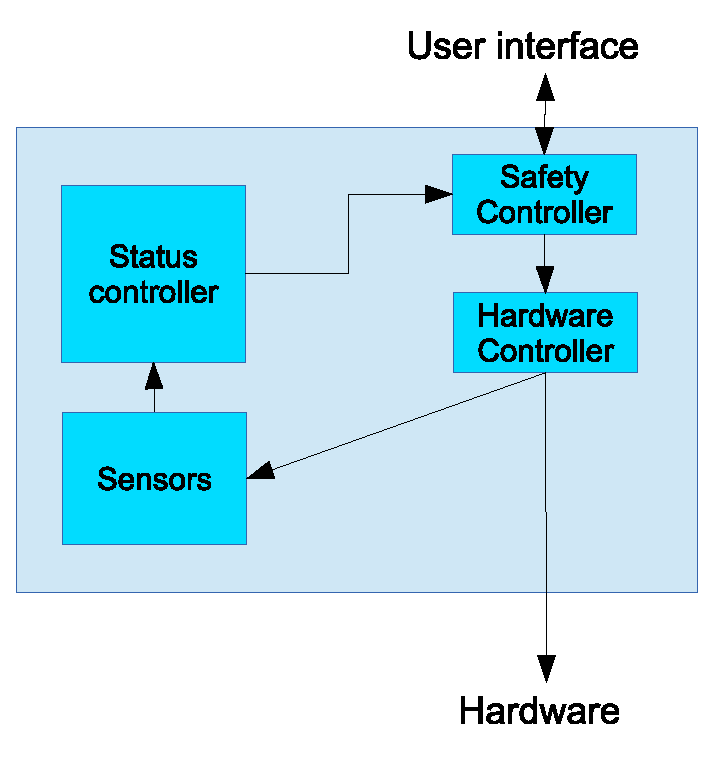
\includegraphics[width=0.6\textwidth]{./images/system-architecture.eps}
		\caption{The system architecture, components and their interactions}
		\label{fig:arch}
		\end{center}
	\end{figure}
	
	
	\section{Safety controller}
		The safety controller is embedded between the user interface and the hardware
		controller. 
		Its responsibility is to check whether the user's requests do not
		lead to an unsafe situation. 
		The checking of preconditions is performed based on the current state of the bridge.
		This information is retrieved from the status controller which is discussed in \cref{sec:arch:status}.
		
		If there is a threat to the safety it should not pass the request to the hardware controller and return an error message to the environment. 
		When the request is no threat to the safety of the system it should be forwarded to the hardware controller.
	
	
	
	\section{Status controller} \label{sec:arch:status}
		The status controller polls the sensors and aggregates information to determine the
		state of the bridge, whose main goal is to deal with inconsistent sensor data or a failure of a sensor. 
		When it is impossible to deduce correct information it should return an error to the user interface.
		It should also forward any other sensor errors that occur in the system like a error from the motor's sensor.
	
	
	
	\section{Hardware controller}
		All validated requests from the user are forwarded by the safety controller to the hardware controller.
		This component controls the hardware. 
		It can control the (pre-)signs, move the barriers, (dis)engage the locking pins and brakes, and control the engine. 
		The requests for opening and closing the bridge involve several actions of the system, which are issued by the safety controller in the right order. 
		The right order of these actions are specified in \cref{tbl:actionorder}
	
	\begin{table}[!htbp]
		\begin{center}
		\begin{tabular}{| l | l | l |}
			\hline
			Order & Opening the bridge 	& Closing the bridge	\\
			\hline
			1 & doPins(switch\_off) 	&	doMotor(motor\_down)	\\
			2 & doBrakes(switch\_off)	&	doBrakes(switch\_off)	\\
			3 & doMotor(motor\_up)		&	doMotor(motor\_stop)\\
			4 & doBrakes(switch\_on)	&	doBrakes(switch\_on)\\
			5 & doMotor(motor\_stop)	&	doPins(switch\_on)	\\
			\hline
		\end{tabular}
		\caption{The right order of actions for opening and closing the brigde.}
		\label{tbl:actionorder}
		\end{center}
	\end{table}

	\section{Sensors}
		The sensors component persists sensor information for four pre-signs, four stop-signs and the five other sensors. 
		The values returned by the sensors are not necessarily correct.
		It is the responsibility of the Status Controller to poll these sensors and handle any errors.

